\section{What is \BoxLib?}

\BoxLib\ is a software library containing all the functionality to write parallel, 
block-structured adaptive mesh refinement (AMR) applications.  \BoxLib\ was developed 
at the Center for Computational Sciences and Engineering (CCSE) at Lawrence Berkeley 
National Laboratory.  Further information can be found by contacting Mike Lijewski 
of CCSE at {\tt MJLijewski@lbl.gov} or by visiting our webpage
at {\tt https://ccse.lbl.gov/}.  Key features of \BoxLib\ include:

\begin{itemize}
\item Support for block-structured AMR with optional subcycling in time
\item Support for cell-centered, face-centered and node-centered data
\item Support for hyperbolic, parabolic and elliptic solves on hierarchical grid structure
\item C++ and Fortran90 versions
\item Supports hybrid programming model with MPI and OpenMP
\item Basis of mature applications in combustion, astrophysics, cosmology, and porous media
\item Demonstrated scaling of linear solvers to 100,000 processors and 
      hydrodynamics to over 200,000 processors
\item Freely available to interested users on our website
\item The plotfile format generated by \BoxLib\ can be read by {\tt VisIt}, {\tt AmrVis},
      and {\tt yt}.
\end{itemize}

\subsection{Overview}

The fundamental parallel abstraction is the \MultiFab\, which holds the data on the 
union of grids at a level.  A \MultiFab\ is composed of fortran array boxes 
(i.e., \FArrayBox\ or \Fab~s); each \Fab\ is an array of data on a single grid. 
During each \MultiFab\ operation the \Fab~s composing that \MultiFab\ are distributed 
among the cores.  \MultiFab~s at each level of refinement are distributed 
independently.  The software supports two data distribution schemes, as well as a 
dynamic switching scheme that decides which approach to use based on the number of 
grids at a level and the number of processors.  The first scheme is based on a 
heuristic knapsack algorithm; the second is based on the use of a Morton-ordering 
space-filling curve.  \MultiFab\ operations are performed with an owner computes rule 
with each processor operating independently on its local data.  For operations that 
require data owned by other processors, the \MultiFab\ operations are preceded by a 
data exchange between processors.  Each processor contains meta-data that is needed 
to fully specify the geometry and processor assignments of the \MultiFab~s. At a 
minimum, this requires the storage of an array of boxes specifying the index space 
region for each AMR level of refinement.  The meta-data can thus be used to 
dynamically evaluate the necessary communication patterns for sharing data amongst 
processors, enabling us to optimize communications patterns within the algorithm.
One of the advantages of computing with fewer, larger grids in the hybrid 
OpenMP--MPI approach (see below) is that the size of the meta-data is substantially 
reduced.

\subsection{Hybrid Parallelism}

The basic parallelization strategy uses a hierarchical programming approach for 
multicore architectures based on both MPI and OpenMP. In the pure-MPI instantiation, at 
least one grid at each level is distributed to each core, and each core communicates 
with every other core using only MPI.  In the hybrid approach, where on each socket/node 
there are $n$ cores which all access the same memory, we can instead have one larger 
grid per socket/node, with the work associated with that grid distributed among the $n$ 
cores using OpenMP.

\subsection{Parallel I/O}

Data for checkpoints and analysis are written in a self-describing format that consists 
of a directory for each time step written. Checkpoint directories contain all necessary 
data to restart the calculation from that time step. Plotfile directories contain data 
for postprocessing, visualization, and analytics, which can be read using AmrVis, a 
customized visualization package developed at LBNL for visualizing data on AMR grids, or 
VisIt. Within each checkpoint or plotfile directory is an ASCII header file and 
subdirectories for each AMR level. The header describes the AMR hierarchy, including 
number of levels, the grid boxes at each level, the problem size, refinement ratio 
between levels, step time, etc. Within each level directory are the MultiFab files for 
each AMR level. Checkpoint and plotfile directories are written at user-specified intervals. 

Restarting a calculation can present some difficult issues for reading data efficiently. 
In the worst case, all processors would need data from all files. If multiple processors 
try to read from the same file at the same time, performance problems can result, with 
extreme cases causing file system thrashing. Since the number of files is generally not 
equal to the number of processors and each processor may need data from multiple files, 
input during restart is coordinated to efficiently read the data. Each data file is only 
opened by one processor at a time. The IOProcessor creates a database for mapping files 
to processors, coordinates the read queues, and interleaves reading its own data. Each 
processor reads all data it needs from the file it currently has open. The code tries to 
maintain the number of input streams to be equal to the number of files at all times. 
Checkpoint and plotfiles are portable to machines with a different byte ordering and 
precision from the machine that wrote the files. Byte order and precision translations 
are done automatically, if required, when the data is read.

\subsection{Scaling}

In Figure \ref{fig:scaling} we present weak scaling results for several of our codes on 
the Cray XT5 Jaguarpf at OLCF. Jaguarpf has two hex-core sockets on each node. We assign 
one MPI process per node and spawn a single thread on each of the 12 cores. Results are 
shown for our compressible astrophysics code, {\tt CASTRO}; the low Mach number code, 
{\tt MAESTRO}; and our low Mach number combustion code, {\tt LMC}. In the {\tt MAESTRO} 
and {\tt CASTRO} tests, we simulate a full spherical star on a 3D grid with one refined 
level (2 total levels).  {\tt LMC} is tested on a 3D methane flame with detailed chemistry 
using two refined levels. {\tt MAESTRO} and {\tt LMC} scale well to 50K-100K cores, 
whereas {\tt CASTRO} scales well to over 200K cores. The overall scaling behavior 
for {\tt MAESTRO} and {\tt LMC} is not as close to ideal as that of {\tt CASTRO} 
due to the communication-intensive linear solves performed at each time step. However, 
these low Mach number codes are able to take a much larger time step than explicit 
compressible formulations in the low Mach number regime. 
%%%%%%%%%%%%%%%%%%%%%%%%%%%%%%%%%%%%%
\begin{figure}[h]
\centering
\includegraphics[width=3in]{./BoxLib/castro_scaling}
\includegraphics[width=3in]{./BoxLib/maestro_scaling}
\includegraphics[width=3in]{./BoxLib/lmc_scaling}
\caption{\label{fig:scaling}Weak scaling results for {\tt CASTRO}, {\tt MAESTRO}, and
{\tt LMC} on the Cray XT5 Jaguarpf at OLCF.}
\end{figure}
%%%%%%%%%%%%%%%%%%%%%%%%%%%%%%%%%%%%%

\section{\BoxLib\ Directory Structure}

\BoxLib\ is the base directory in a hierarchy of subdirectories that
support parallel, block-structured AMR applications in C++ and fortran.
A schematic of the \BoxLib\ directory structure is shown in Figure 
\ref{fig:boxlib_directory}.
%%%%%%%%%%%%%%%%%%%%%%%%%%%%%%%%%%%%%
\begin{figure}[h]
\centering
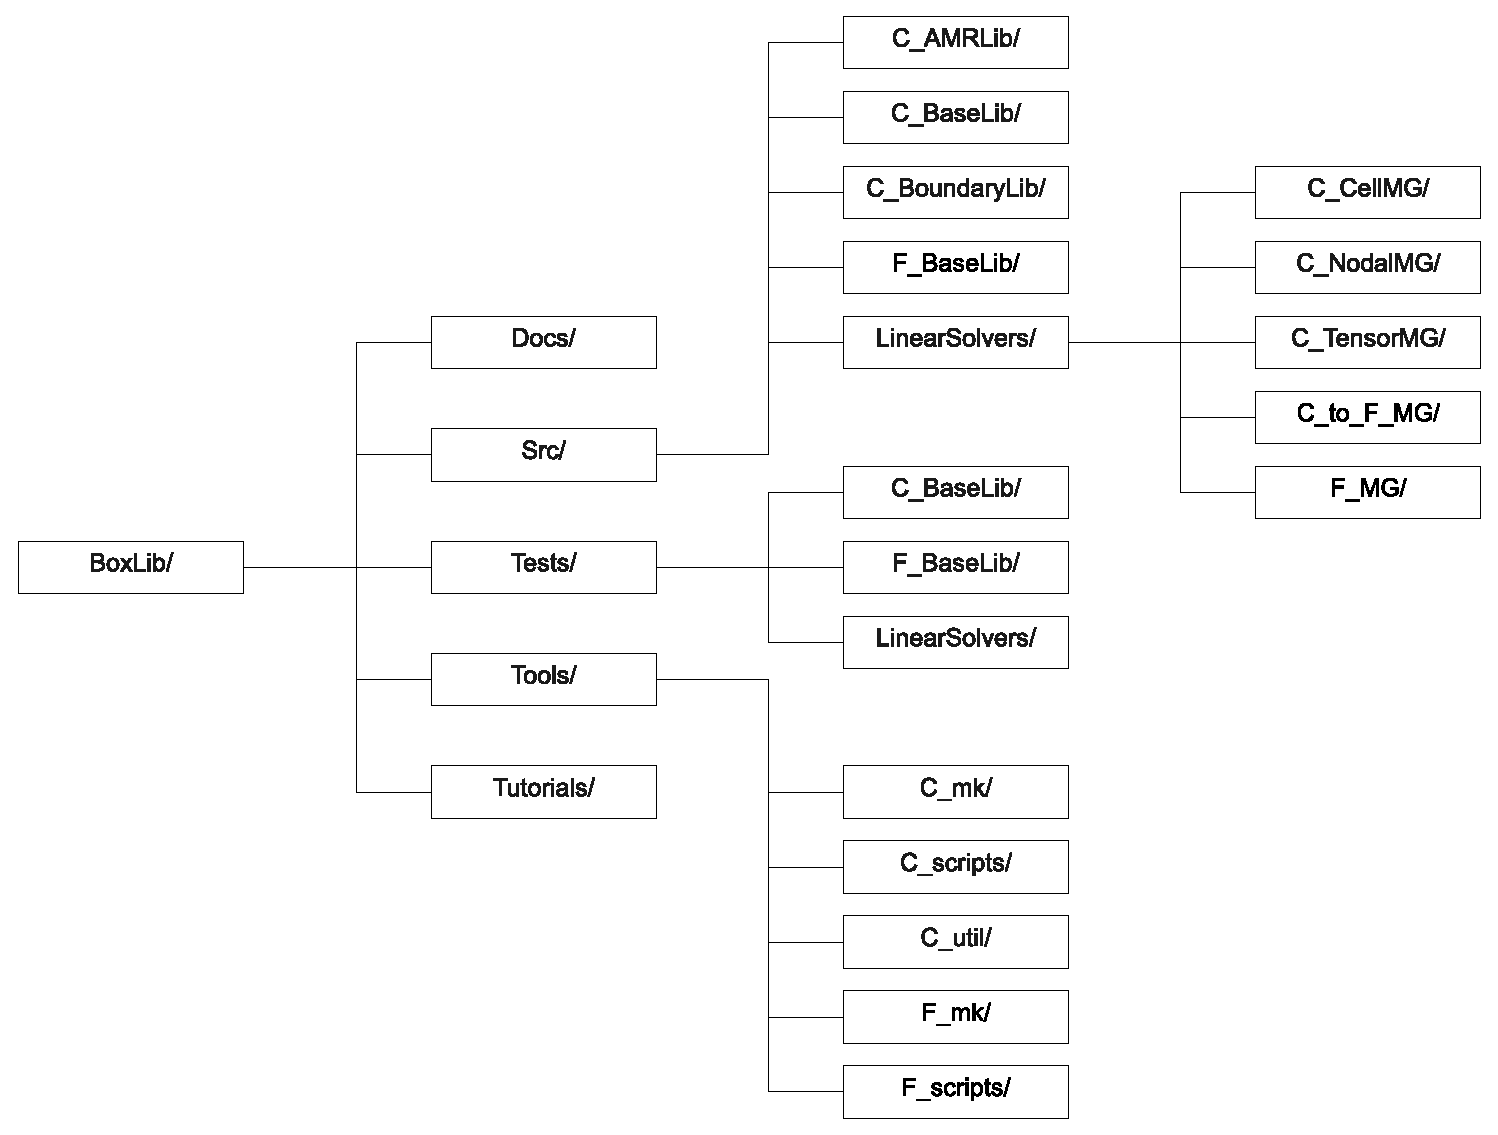
\includegraphics[width=6.5in]{./BoxLib/boxlib_directory_bw2}
\caption{\label{fig:boxlib_directory}\BoxLib\ directory structure.}
\end{figure}
%%%%%%%%%%%%%%%%%%%%%%%%%%%%%%%%%%%%%

\begin{itemize}

\item {\tt Docs/}

Contains the \BoxLib\ User's Guide.

\item {\tt Src/}

  \begin{itemize}

    \item {\tt C\_AMRLib/}
    \item {\tt C\_BaseLib/}
    \item {\tt C\_BoundaryLib/}
    \item {\tt F\_BaseLib/}
    \item {\tt LinearSolvers/}

    \begin{itemize}

      \item {\tt C\_CellMG/}
      \item {\tt C\_NodalMG/}
      \item {\tt C\_TensorMG/}
      \item {\tt C\_to\_F\_MG/}
      \item {\tt F\_MG/}

    \end{itemize}

  \end{itemize}

\item {\tt Tests/}

  \begin{itemize}

  \item {\tt C\_BaseLib/}
  \item {\tt F\_BaseLib/}
  \item {\tt LinearSolvers/}

  \end{itemize}

\item {\tt Tools/}

  \begin{itemize}

  \item {\tt C\_mk/}

  The generic Makefiles that store the C++ compilation flags for
  various platforms.

  \item {\tt C\_scripts/}

  Some simple scripts that are useful for building, running,
  maintaining codes in \BoxLib.

  \end{itemize}

  \item {\tt C\_Util/}
  \item {\tt F\_mk/}
  \item {\tt F\_scripts/}

\item {\tt Tutorials/}

\end{itemize}

\section{\BoxLib\ Data Structures}

\BoxLib\ contains the most fundamental objects used to construct block-structured
AMR applications.  The objects in \BoxLib\ support structured
grid adaptive mesh refinement (AMR), i.e. in a single calculation
different regions of the domain can have different spatial resolutions.  
At each level of refinement, the region covered by that level is broken
into boxes, or grids.  The entire computational domain is covered by
the coarsest (base) level of refinement, often called level 0. 
Higher levels of refinement have finer zones by a ``refinement ratio''
of either 2 or 4.  Only a portion of the domain may
be covered by the higher levels of refinement.  

The grids are properly nested, in the sense that the union of grids
at level $\ell+1$ is contained in the union of grids at level $\ell$.
Furthermore, the containment is strict in the sense that,
except at physical boundaries,
the level $\ell$ grids are large enough to guarantee that there is
a border at least $n_{\rm proper}$ level $\ell$ cells wide surrounding each level
$\ell +1$ grid (grids at all levels are allowed to extend to the physical
boundaries so the proper nesting is not strict there).
For parallel computations, the boxes are distributed to processors, in
a fashion designed to put roughly equal amounts of work on each
processor (load balancing).

On a grid, the data can be stored at cell-centers, on a face/edge, or
on the corners.  In \BoxLib\, data that is on an edge is termed `nodal'
in that direction (see Figure~\ref{fig:dataloc}).  Data that is on the
corners is nodal in all spatial directions.  In our Parallel applications, 
the state data (velocity, density, species $\ldots$) is generally
cell-centered.  Fluxes are nodal in the direction they represent.
A few quantities are nodal in all directions (e.g.\ the pressure in
the low Mach number projection methods).

%%%%%%%%%%%%%%%%%%%%%%%%%%%%%%%%%%%%%
\begin{figure}[h]
\centering
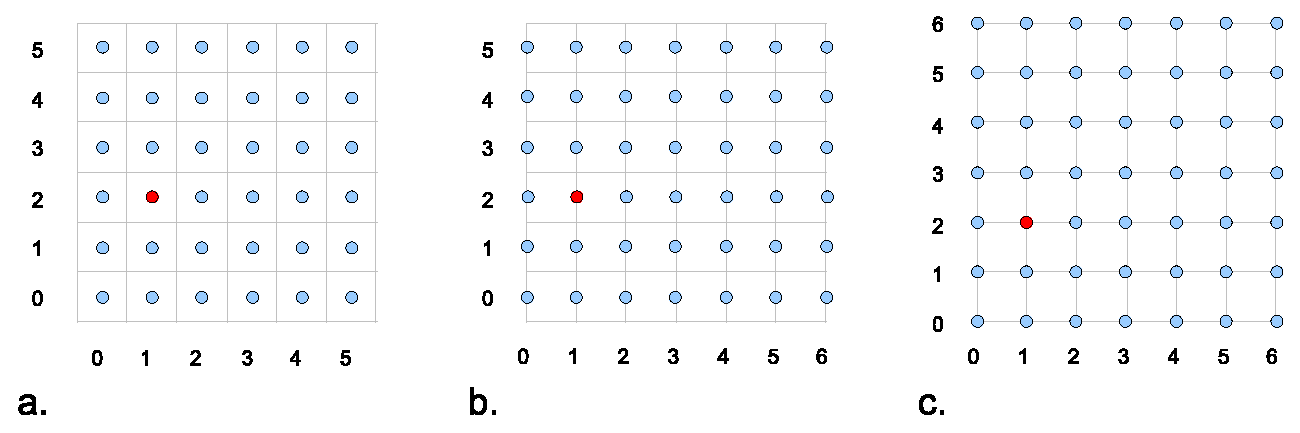
\includegraphics[width=6.5in]{./BoxLib/data_loc2}
\caption{\label{fig:dataloc} Some of the different data-centerings:
(a) cell-centered, (b) nodal in the $x$-direction, and (c) nodal in
both the $x$- and $y$-directions.  Note that for nodal data, the
integer index corresponds to the lower boundary in that direction.
In each of these centerings, the red point has the same indices:\ (1,2).
Not shown is the case where data is nodal in the $y$-direction only.}
\end{figure}
%%%%%%%%%%%%%%%%%%%%%%%%%%%%%%%%%%%%%

To simplify the description of the underlying AMR grid, \BoxLib\
provides a number of classes.  We briefly summarize some of the major
classes below.

First, note that when a Parallel application is compiled and linked,
the number of spatial dimensions (1,2 or 3), {\bf DIM},
 of the code must be specified.  The code that will be
built is specifically designed to run only with that number of dimensions.
(This is unlike the fParallel data structures in which we build
dimension-independent code at compile-time.)

\subsection{\IntVect}

\IntVect~s are n-tuples of integers that are used to define
indices in space.  An example of an \IntVect\ in 2D would
be (3,5).

\subsection{\BoxType}

A \BoxType\ is simply a rectangular domain in space.  Note that \BoxType~s
do not hold any data themselves. A box basically contains
only the indices of its low end and high end as well as a type 
(cell-centered, edge-centered, or nodal).

%%%%%%%%%%%%%%%%%%%%%%%%%%%%%%%%%%%%%
\begin{figure}[h]
\centering
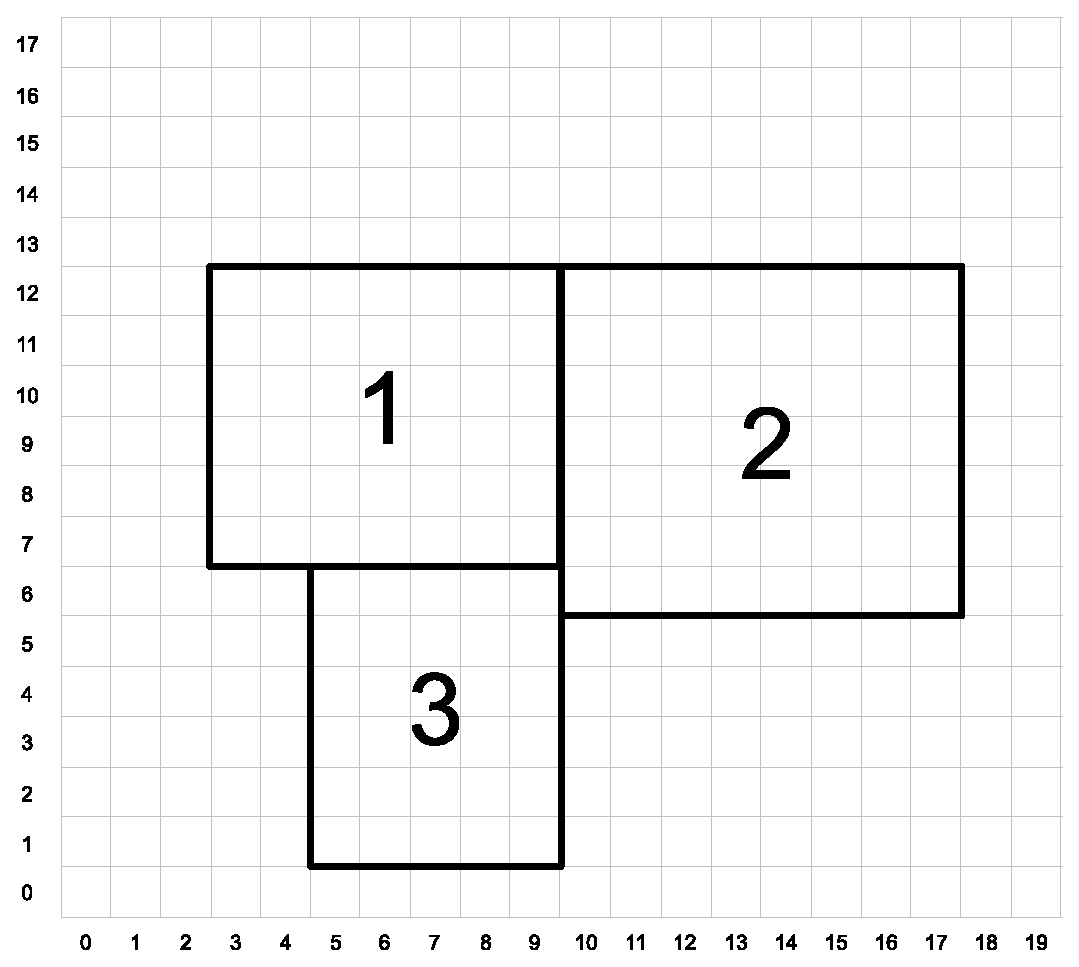
\includegraphics[width=4.0in]{./BoxLib/index_grid2}
\caption{\label{fig:boxes} Three boxes that comprise a single level.
At this resolution, the domain is 20$\times$18 zones.  Note that the
indexing in \BoxLib\ starts with $0$.}
\end{figure}
%%%%%%%%%%%%%%%%%%%%%%%%%%%%%%%%%%%%%

The computational domain is divided into boxes.  The collection of
boxes with the same resolution comprise a level.
Figure~\ref{fig:boxes} shows three boxes at the same level of
refinement.  The position of the boxes is with respect to a global
index space at that level.  For example, box 1 in the figure has 
{\tt lo} = (3,7) and {\tt hi} = (9,12).  

For a \BoxType\ {\bf bx},
you can access the indices {\bf bx} using the 

\begin{itemize}
\item {\tt smallEnd}  -- for box 1 above this would return the \IntVect\ (3,7)
\item {\tt bigEnd} -- for box 1 above this would return the \IntVect\ (9,12)
\end{itemize}

\subsection{\BoxArray}

A \BoxArray\ is an array of boxes.   The size of the array is the 
number of boxes in the \BoxArray.

\subsection{\FArrayBox}

A \FArrayBox\ (or \Fab) is a ``Fortran Array Box'' that holds data.  It contains the
\BoxType\ that it is built on as well as a pointer to the data 
that can be sent to a Fortran routine.
 
To build a \Fab\ you must specify the \BoxType\ and the number of components.
For example, the section of code below builds a \Fab\ called {\tt myfab}
that has two components of data defined on the box from (0,0) to (31,15).

\begin{verbatim}
IntVect iv_lo(0,0);
IntVect iv_hi(31,15);
Box bx(iv_lo,iv_hi);
FArrayBox myfab;
myfab.define(bx,2);
\end{verbatim}

In Parallel, we don't usually deal with \Fab~s alone, but rather
through \MultiFab~s, described next.

\subsection{\MultiFab}

A \MultiFab\ is a collection of \Fab~s at the same level of
refinement.  A \MultiFab\ is defined using a \BoxArray,
number of components, and number of ``ghost'' calls that each box
will have.  Note that a \Fab\ has no concept of ghost cells, it
merely has a single box that identifies it.  A \MultiFab\ has
a "valid" region that is defined by the \BoxArray.  In addition,
each \Fab\ in the \MultiFab\ is built large enough to hold data
on the box associated with it {\it grown by ngrow ghost cells.}

If we had a \BoxArray, {\tt myba}, then we could define a \MultiFab\ as"

\begin{verbatim}
MultiFab mymf(myba,2,1);
\end{verbatim}

This \MultiFab\ has two components of data and each \Fab\ in the \MultiFab\ contains ghost cells one row wide in all directions outside the box from the \BoxArray.

